% !TEX root = ../thesis.tex

\chapter{AVPipe视频流处理框架的设计与实现}
为了解决在\ref{moti_obj}中所述的目标,我们设计了Accel-Video Pipe(AVPipe),一套模块化的对基于DAG计算图的视频流处理提供开发便捷以及加速优化的编程框架。在这一章中,我们将具体介绍AVPipe的设计逻辑与框架结构。

\section{AVPipe的设计逻辑}
% 先讲逻辑抽象:
%   以 数据流 ,数据处理的分离。由管道将数据与不同处理模块相连接。
% 再讲各部分是如何设计的 
针对视频流处理任务在多阶段有依赖的较复杂计算流程,我们需要使AVPipe编程框架能够对整个智能视频处理流程进行合理的抽象。\par
视频流处理中,数据是不断地由起始节点(source),经过一步步的计算流向汇聚节点(sink)的。这一过程中,数据是在整个计算流程中持续变化的,此外,这些产生的数据也存在着时序上的依赖关系。另一方面,处理流程图中的每一个计算节点所承担的计算任务是固定的。为了对计算流程图进行管理与优化,所有计算模块需要有通过一套简单的、统一的类(class)或结构(struct)来进行封装。\par
基于以上两方面的考虑,我们将AVPipe中的数据与数据处理单元分离开来,分别抽象为StreamPacket和PipeProcessor。为实现数据与数据处理单元之间的交互,我们又建立了对数据流的抽象Stream。数据流(Stream)将不同数据处理单元(PipeProcessor)连接成一个整体,为数据(StreamPacket)提供了流动的载体与指引,使得数据可以有序地、高效地流向各个处理单元。 对数据,数据流以及数据处理单元的抽象是AVPipe框架的主要设计逻辑,图\ref{fig:base_struct}直观展示了这三者在AVPipe中的关系。接下来我们会逐一介绍这三部分的具体设计。
\begin{figure}[htp]
    \centering
    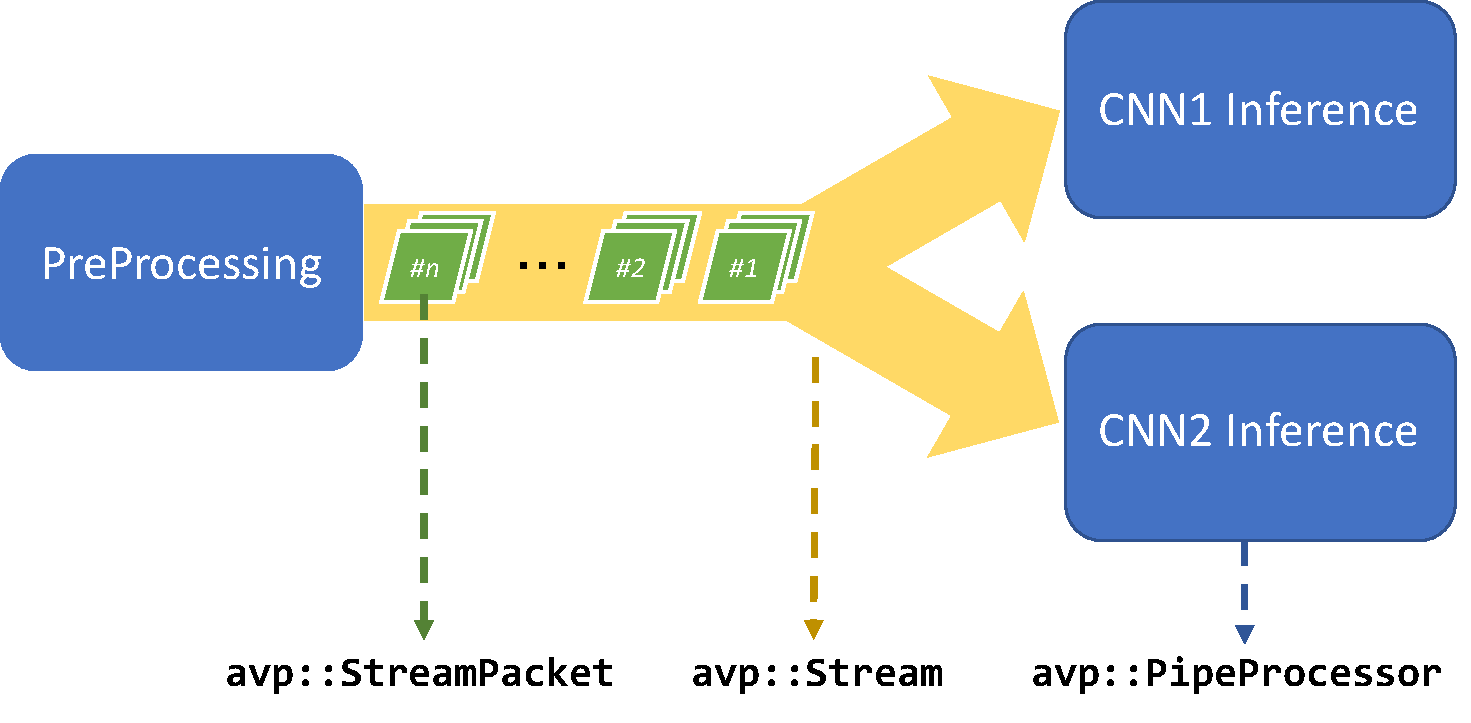
\includegraphics[width=0.8\textwidth]{figure/avp_base_struct.pdf}
    \caption{AVPipe基本抽象之间的关系}
    \label{fig:base_struct}
\end{figure}
\subsection{数据包StreamPacket}
StreamPacket中包含了视频流处理流程中的待处理数据。每个StreamPacket只表示单一类型的数据(如图片,矩阵或张量等)。
为了保证数据的同步与时序,每个StreamPacket都有一个时间戳(timestamp)来记录自己的创建时间步,同一时间步的所有StreamPacket需要在同一处理流程周期中完成。
考虑到某些数据处理步骤可能会在同一时间步中产生多个处理结果,数据在StreamPacket中需要以列表的形式来进行维护。某些数据处理过程也可能会由于没有满足条件而产生空的数据包,空数据包作为作为处理流程中的正常产物,StreamPacket仍然需要对其提供必要的处理逻辑。此外,由于整个AVPipe的数据处理是围绕着StreamPacket来进行的,当整个处理流程结束时,需要依赖StreamPacket的传播来告知每个数据单元来停止运行,因此除了空数据包外,StreamPacket还需提供携带结束信息的终止数据包。
\subsection{数据流Stream}\label{ch4:design_stream}
Stream是StreamPacket的载体,其主体需要存在一个队列结构来有序存取StreamPacket。另一方面,Stream又有着连接PipeProcessor的作用,由于同一个人数据可能会被多个步骤利用,因此同一个Stream可能会同时连接多个PipeProcessor(如图\ref{fig:base_struct})。考虑到多个PipeProcessor可能会多线程同时运行,Stream需要为此提供一定的同步与阻塞机制,以免数据的错位与误读。
当数据包完成在PipeProcessor被使用并完成处理时,PipeProcessor会向Stream发送该数据包的释放请求,Stream要能判断该数据包是否被所连接的所有PipeProcessor全部使用,当且仅当所有PipeProcessor都使用了该数据包后,数据包才会从Stream中安全释放。
有时候,由于数据生产速度会超过数据消费速度,数据包StreamPacket会不断地积累在Stream中而不能及时处理,最终导致大量内存的不必要消耗。为此,Stream还需要提供一个长度或容量的限制,结合阻塞机制来防止数据包的聚积。

\subsection{数据处理单元PipeProcessor}\label{ch4:design_proc}
PipeProcessor是对视频流处理中各个计算步骤的抽象。PipeProcessor从其连接的输入Stream中拿到数据进行处理,将计算结果放入输出Stream中。PipeProcessor根据根据其输入输出的方式不同,可以分为三类:
\begin{enumerate}
    \item 数据处理型(Process):既有输入数据,也有输出数据。视频流处理中的绝大多数多数处理模块的属于这一形式;
    \item 数据起源型(Source):只有输出数据。主要用于获取或产生数据源(如视频摄像头的捕捉或视频文件的读取)供接下来的处理使用;由于Source节点为每一次处理的起点,当视频处理任务结束时,需要由其产生终止数据包来传播给其他所有计算节点。
    \item 数据汇聚型(Sink):只有输入数据。主要用于汇集视频处理的结果,用以保存或窗口展示。当所有的Sink节点都收到终止数据包时,这意味着所有计算节点都收到了终止信号,整个视频处理流程就会停止运行。
\end{enumerate}
流处理中的不同处理模块都是对PipeProcessor的继承与实现。不同模块可以定义自己所需的变量或内存,其实际计算则是通过重载PipeProcessor中的运行接口(\texttt{run})来实现的,在这个运行接口中只需要定义处理相关的计算即可。对于运行的前的准备,输入数据的检查,时间戳的校对则是由PipeProcessor内不另一个接口来实现的(\texttt{process}),\texttt{process}要能检查输入的有效性。当输入为空数据包时,\texttt{process}在默认情况\footnote{部分输入数据为空时,数据处理逻辑也有可能产生非空的输出。如对检测结果的在检测帧上渲染时,检测结果可能为空。}下会直接返回空的输出数据,而不调用\texttt{run}接口。\texttt{process}对终止数据包也会有类似的处理,不再赘述。总之,在实际使用中,我们不能直接调用\texttt{run}的接口,
而是通过调用对\texttt{run}再次封装的\texttt{process}接口。这样的设计一方面可以提高代码运行的可靠性,另一方面可以简化不同模块计算流程的实现。

\section{AVPipe的框架实现}\label{ch4:impl}
在介绍了AVPipe主体的设计逻辑后,我们将在本小节关注框架实现中存在的需要特别考虑的内容,同样围绕着数据包,数据流以及数据处理单元这三大部分进行展开。
% 讲 Mat 与 Tensor的 整合
\subsection{StreamPacket中数据格式的整合}
针对\ref{ch3:problems}中提到的数据格式在不同处理步骤中的不能不统一使用的问题,我们期望StreamPacket的封装能够在这方面带来改善。对视频流处理这一类任务来说,我们可以将处理流程中可能涉及到处理数据的格式进行总结。通过调研不同视频流处理任务发现,所涉及的数据处理主要包含两种数据格式:(1)图像的矩阵数据,数据主要以OpenCV的Mat格式来参与传统的数字图像处理运算,如图像的裁剪,缩放,仿射变化等,但是Mat数据有维度的限制,如\ref{ch2:framewk}中所说,它不能很好地处理高维张量数据;(2)机器学习相关的张量数据,张量数据主要用于神经网络的计算以及相关的后处理操作中,张量数据在各个深度学习推理引擎中的表示不尽相同,对高维张量的操作难易程度也不尽相同。通过以上分析,我们可以确定的是StreamPacket需要同时对图像矩阵以及高维张量提供良好的支持,接下来我们要考虑具体实现实现方式。\par

首先,在关于图像矩阵的处理上,OpenCV是受业界普遍认可的通用数字图像处理库。因此,在StreamPacket中的数据提供直接的\texttt{cv::Mat}形式的数据存储是对传统数字图像处理操作最友好的支持。
再来看对高维张量的处理。由于这方面的需求是在近些年由机器学习技术的快速发展而兴起的,这使得目前在C/C++语言下没有一个像Python中NumPy那样的,开发完善的,普遍使用的针对高维数据的科学计算库,从而导致不同的机器学习框架会各自为阵,开发仅供本框架使用的数据格式以及数据处理方式,如TVM所使用的DLPack\cite{dlpack}库,PyTorch所使用的ATen库。通过实际使用和测试发现,PyTorch/Caffe2所使用的ATen张量库有最为完善的张量定义以及操作算子,其类似Python的数据操作与丰富的开发文档也带来了出色的使用体验。我们也因此将ATen库中的张量格式\texttt{at::Tensor}做为AVPipe主要支持的张量格式。\par

通过以上分析,我们确立了对\texttt{cv::Mat}以及\texttt{at::Tensor}这两种数据格式的支持,我们现在开始考虑如何对这两部分在StreamPacket中进行有机结合。考虑到OpenCV与LibTorch都是提供预编译的开源库,我们并不打算对这两个库的底层代码进行修改以实现操作的互通,这在工程难度以及通用性上都不可行。于是我们考虑在StreamPacket中同时保留\texttt{Mat}和\texttt{Tensor}的数据队列。通常情况下,一个Stream对应的StreamPacket都是同一个类型的,也就是说,\texttt{Mat}和\texttt{Tensor}两者中一般只有一个保存有待处理数据。PipeProcessor在生成数据时,也会规定数据将在StreamPacket中以哪种方式保存,这使得StreamPacket在管理内部数据时只需关注它所对应形式的数据。
此外,我们也在StreamPacket的内部,通过内存指针引用的方式,提供了\texttt{Mat}和\texttt{Tensor}相互类型转换的方法,为不同应用场景提供便利。

% 同步以及其他特殊情况的考虑
\subsection{Stream中数据的同步与管理}
在\ref{ch4:design_stream}中,我们介绍了Stream的设计逻辑。在这一部分里,我们主要说明在Stream实现过程中要考虑的关键点。由于Stream本质是存放AVPipe数据包的一个队列,因此Stream直接继承STL(C++标准模版库)中的deque\footnote{\url{http://www.cplusplus.com/reference/deque/deque/}},并在此基础上提供功能的完善与拓展。\par

对deque拓展的核心在于为其添加多线程的数据同步与阻塞机制,在这里我们使用C++11标准提供的多线程相关函数库来进行实现。具体来说,我们在Stream中定义了一个互斥锁变量(mutex\footnote{\url{https://en.cppreference.com/w/cpp/thread/mutex}})\texttt{consumeMutex}来实现数据的同步,两个条件变量(condition variable\footnote{\url{https://en.cppreference.com/w/cpp/thread/condition_variable}})\texttt{loadCond}和\texttt{spaceCond}分别实现对读取空队列和超队列容量存储的阻塞。\par

\texttt{consumeMutex}在数据释放时使用。由于在数据释放时需要判断是否该数据包已经被所有的下游依赖计算节点全部使用(通过判断统计变量\texttt{num\_consume}来实现),可能存在多个线程同时判断该数据包是否完成处理的竞争条件(race condition)。为保证操作的一致性与原子性,需要在数据释放操作上加互斥锁。\par

\texttt{loadCond}和\texttt{spaceCond}都是使用条件变量的机制,当发现当前线程不满足的所设置的判断条件时,将线程进行休眠,直到满足条件后,由其他线程通过条件变量唤醒该线程。比如某处理线程在读取Stream时发现队列为空,这时\texttt{loadCond}会将该线程挂起,直到有新的数据包载入该Stream中时,进行数据包载入的线程就会向\texttt{loadCond}进行告知(\texttt{notify\_one()}),从而唤醒挂起的线程,继续读取数据。\texttt{spaceCond}则是在数据包载入Stream时由于队列容量以达到上线而造成的线程挂起,当队列中有数据包被释放时,该线程又会被唤醒,继续进行数据载入。\par

图\ref{fig:stream_code}展示了Stream对以上问题的实际代码实现,这三个函数由同一个互斥量\texttt{consumeMutex}关联在一起,保证了代码执行的正确性。
这些对Stream实现中关于多线程的考虑在很多编程语言如Java与Python中都有类似的实现。我们对C++标准库的队列的改造使得它满足了我们在视频流处理中的需求。
% coupleStream 实现Stream在不同队列中非同步的数据使用?
% 考虑加点代码片段?

\begin{figure}[!htp]
  \centering
  \begin{subfigure}{0.32\textwidth}
    \centering
    
\begin{codeblock}[language=C, basicstyle=\ttfamily\tiny]
void loadPacket(StreamPacket& packet) 
{
    num_consume = numConsume;
    unique_lock<std::mutex> locker(consumeMutex);
    spaceCond.wait(locker, [&](){return this->size()<=streamCapacity;});
    push_back(packet);
    locker.unlock();
    loadCond.notify_one();
}
\end{codeblock}

    \caption{loadPacket}
  \end{subfigure}
  \begin{subfigure}{0.32\textwidth}
    \centering
    
\begin{codeblock}[language=C, basicstyle=\ttfamily\tiny]
void releasePacket()
{
    {
        lock_guard<std::mutex> guard(consumeMutex);
        auto it = begin();
        it->numConsume--;
        if(!it->numConsume)
            pop_front();
    }
    spaceCond.notify_one();
}
\end{codeblock}

    \caption{releasePacket}
  \end{subfigure}
  \begin{subfigure}{0.32\textwidth}
    \centering
    
\begin{codeblock}[language=C, basicstyle=\ttfamily\tiny]
StreamPacket& getPacket()
{
    unique_lock<std::mutex> locker(consumeMutex);
    loadCond.wait(locker, [this](){ 
        return !this->empty();
    });
    locker.unlock();
    return front();
}
\end{codeblock}

    \caption{getPacket}
  \end{subfigure}
  
  \caption{Stream中包含同步与阻塞的三个操作的代码片段}
  \label{fig:stream_code}
\end{figure}

% 数据如何在多个计算库运转与整合
% Processor 的实现与自定义
\subsection{PipeProcessor的实现与自定义}
在\ref{ch4:design_proc}中,我们提到了PipeProcessor运行的嵌套关系。所有计算模块都是对PipeProcessor的继承。当一个计算模块要进行数据处理时,首先调用基类PipeProcessor的\texttt{process()}方法,经过输入数据的检查后,\texttt{process}会调用由子类重载的\texttt{run()}方法。在\texttt{run}完成处理后,\texttt{process}方法最后将完成输入数据的释放以及输出数据的转存。接下来我们从PipeProcessor与Stream的连接,具体模块的实现以及模块自定义这三个方面进行讨论。\par
在AVPipe中,PipeProcessor是通过Stream实现相互连接,最终构成一个整体的视频处理流程图的。在上一小节中,我们已经介绍Stream了具体实现,Stream并不直接保存与其相连的PipeProcessor的信息。为了方便PipeProcessor对Stream中数据包的读写,我们将所有的连接信息都被放在了PipeProcessor中。Stream与计算模块的连接是通过PipeProcessor提供的\texttt{bindStream}方法来实现的。为了减少对连接信息的保存和操作开销,我们在PipeProcessor中设置了两个包含Stream指针信息的列表\texttt{inStreams}和\texttt{outStreams}。由于连接信息以列表(STL中的vector\footnote{\url{http://www.cplusplus.com/reference/vector/vector/}})形式保存,这需要我们人为设定其中Stream的保存顺序,这虽然牺牲了部分灵活性,但也为框架的带来了更少的资源开销与额外控制逻辑。
% 非同步 连接以后看需求添加
这一点也会通过在之后\ref{ch4:auto_codegen}中介绍的自动代码生成功能带来一定程度的规范与改进。
\par
由于PipeProcessor这一基类已经完成了绝大部分的控制逻辑,基于此实现的具体计算模块只需完成自身参数的初始化并重载基类中的\texttt{run}方法即可。
计算模块的初始化参数一方面包括在PipeProcessor需要定义的参数如输入输出Stream的数量,计算模块的名称/标签以及数据类型,另一方面也包含运行该计算模块所必要参数如神经网络推理模块需要在初始化导入的模型文件,图像处理模块需要图像目标尺寸等信息。
\texttt{run}方法有两个引用参数\texttt{in\_data\_list}和\texttt{out\_data\_list}分别用来存放本计算的输入和输出数据包列表。输入数据\texttt{in\_data\_list}是由\texttt{process}从本计算模块连接的所有输入Stream中收集得到的(所得的数据列表需要满足时间戳的一致)。\texttt{run}中的数据操作的实现与写一般的数据处理函数并没有太多区别。\par
除了直接向AVPipe中添加新的计算模块外,我们还提供了一个模版计算模块\texttt{TemplateProcessor}。有时候视频流处理任务中会出现一些任务特定的,缺少通用性的计算步骤,如与输入内容密切相关的多路选择器,\texttt{TemplateProcessor}的存在方便了用户快速实现特殊计算模块的构建。\texttt{TemplateProcessor}中保存有一个函数指针用来链接在具体任务代码中实现的数据处理函数。
\texttt{TemplateProcessor}也可以用来构建复合的计算模块,即\texttt{TemplateProcessor}通过引用的形式,在其数据处理流程中直接调用其他模块的\texttt{run}方法,实现复杂的控制逻辑。
模版计算模块的加入更加凸显了AVPipe框架的灵活性与开放性。

\section{AVPipe的自动化工具}
为了进一步提高AVPipe框架的可用性以及易用性,我们还在原始AVPipe的C++框架基础上开发了各种自动化的工具为视频流处理任务的代码开发,性能调试以及运行优化带来便利。这部分代码主要由Python开发,但最终会与AVPipe的C++代码进行互动。
\subsection{配置文件驱动的自动代码生成}\label{ch4:auto_codegen}
如\ref{ch4:impl}中的介绍,我们完成了AVPipe框架的高度模块化的实现。这种模块化极大便利了开发人员对具体视频处理任务在AVPipe框架下的实现,通过不到50行的C++代码即可实现整个视频处理流程的定义与运行。为了更进一步提升AVPipe框架的易用性,使那些对C++开发并不熟悉的用户也可以快速上手AVPipe,我们又为AVPipe提供了配置文件驱动的自动代码生成的功能,不必书写C++代码,仅通过配置文件定义不同计算模块的连接关系以及其他模块参数,我们的自动化工具就会解析配置文件,并生成一个可运行的视频流处理任务的C++文件。\par
在配置文件上,我们使用YAML(YAML Ain't Markup Language\footnote{\url{https://yaml.org/}})格式作为配置定义语法。相比其他配置文件格式,YAML有更好的用户可读性以及语法简洁性。YAML文件在AVPipe中以两种形式存在:(1)计算模块的模版YAML文件,(2)具体视频任务的流程定义YAML文件。模版YAML文件是在定义AVPipe的计算模块时添加的,用来说明该计算模块的默认参数,必须要定义的参数以及需要关联的Stream的数据格式信息,具体形式如图\ref{fig:yaml}所示。任务相关YAML文件是对模版YAML文件的再次补全,设定具体任务的运行参数,并添加\texttt{binding}键值用来描述模块之间的连接关系。\par

\begin{figure}[!htp]
  \centering
  \begin{subfigure}{0.7\textwidth}
    \centering
    
\begin{codeblock}[language=Ruby, basicstyle=\ttfamily\small]
- PipeProcessor: NonMaxSuppression
  includeFile: tensor_compute/det_postprocess.hpp
  label: AVP::REQUIRED
  args:
    clip_thresh: 100.0
    score_thresh: 0.8
    suppression_thresh: 0.3
  inStreams:
  - label: detScoresTensor
  - label: detBoxesTensor
  outStreams:
  - label: outDetsTensor
  - label: outLandMarksTensor
\end{codeblock}
  \end{subfigure}
  
  \caption[AVPipe计算模块的模版YAML文件]{非极大值抑制(NMS)模块在AVPipe中的模版YAML文件。\texttt{AVP::REQUIRED}表示必须由用户定义的参数。}
  \label{fig:yaml}
\end{figure}

对于自动代码生成,由于其涉及较多字符串相关的操作,为简化开发,我们因此选择使用较为灵活的Python语言进行实现。自动代码生成脚本会先对任务相关YAML配置文件进行解析,根据配置参数生成模块的初始化的代码。之后脚本会根据配置文件中的\texttt{binding}键值的信息建立模块之间的连接关系。最后,对计算模块按连接关系进行拓扑排序,按拓扑排序结果生成计算模块的运行代码。编译目标C++文件所需的CMake\footnote{\url{https://cmake.org/}}配置文件,也会在AVPipe的自动化脚本中一并生成。
使用配置文件进行代码生成的方式也为以后使用可视化界面直接通过模块选择与拖拽生成任务处理流程提供了可行性。
% 要不要搞个 算法流程在这里?emmm 算了

\subsection{处理流程可视化与运行时性能分析}\label{ch4:viz_prof}
在\ref{ch4:auto_codegen}中介绍的YAML文件除了可以用于代码的自动生成外,也可用该配置文件可视化整个视频处理流程。此外,可视化工具也可为视频任务的性能分析提供便利。\par

可视化工具同样使用了配置文件中提供的计算模块相互连接的信息,将视频流处理任务所用到的DAG流程图可视化。在这里我们使用Python生成连接图的Graphviz\cite{Gansner00anopen}源文件,然后通过调用Graphviz软件绘制DAG流程图,图\ref{fig:pose_dag}展示了视频姿态检测任务流程的可视化效果。\par

\begin{figure}[tb]
    \centering
    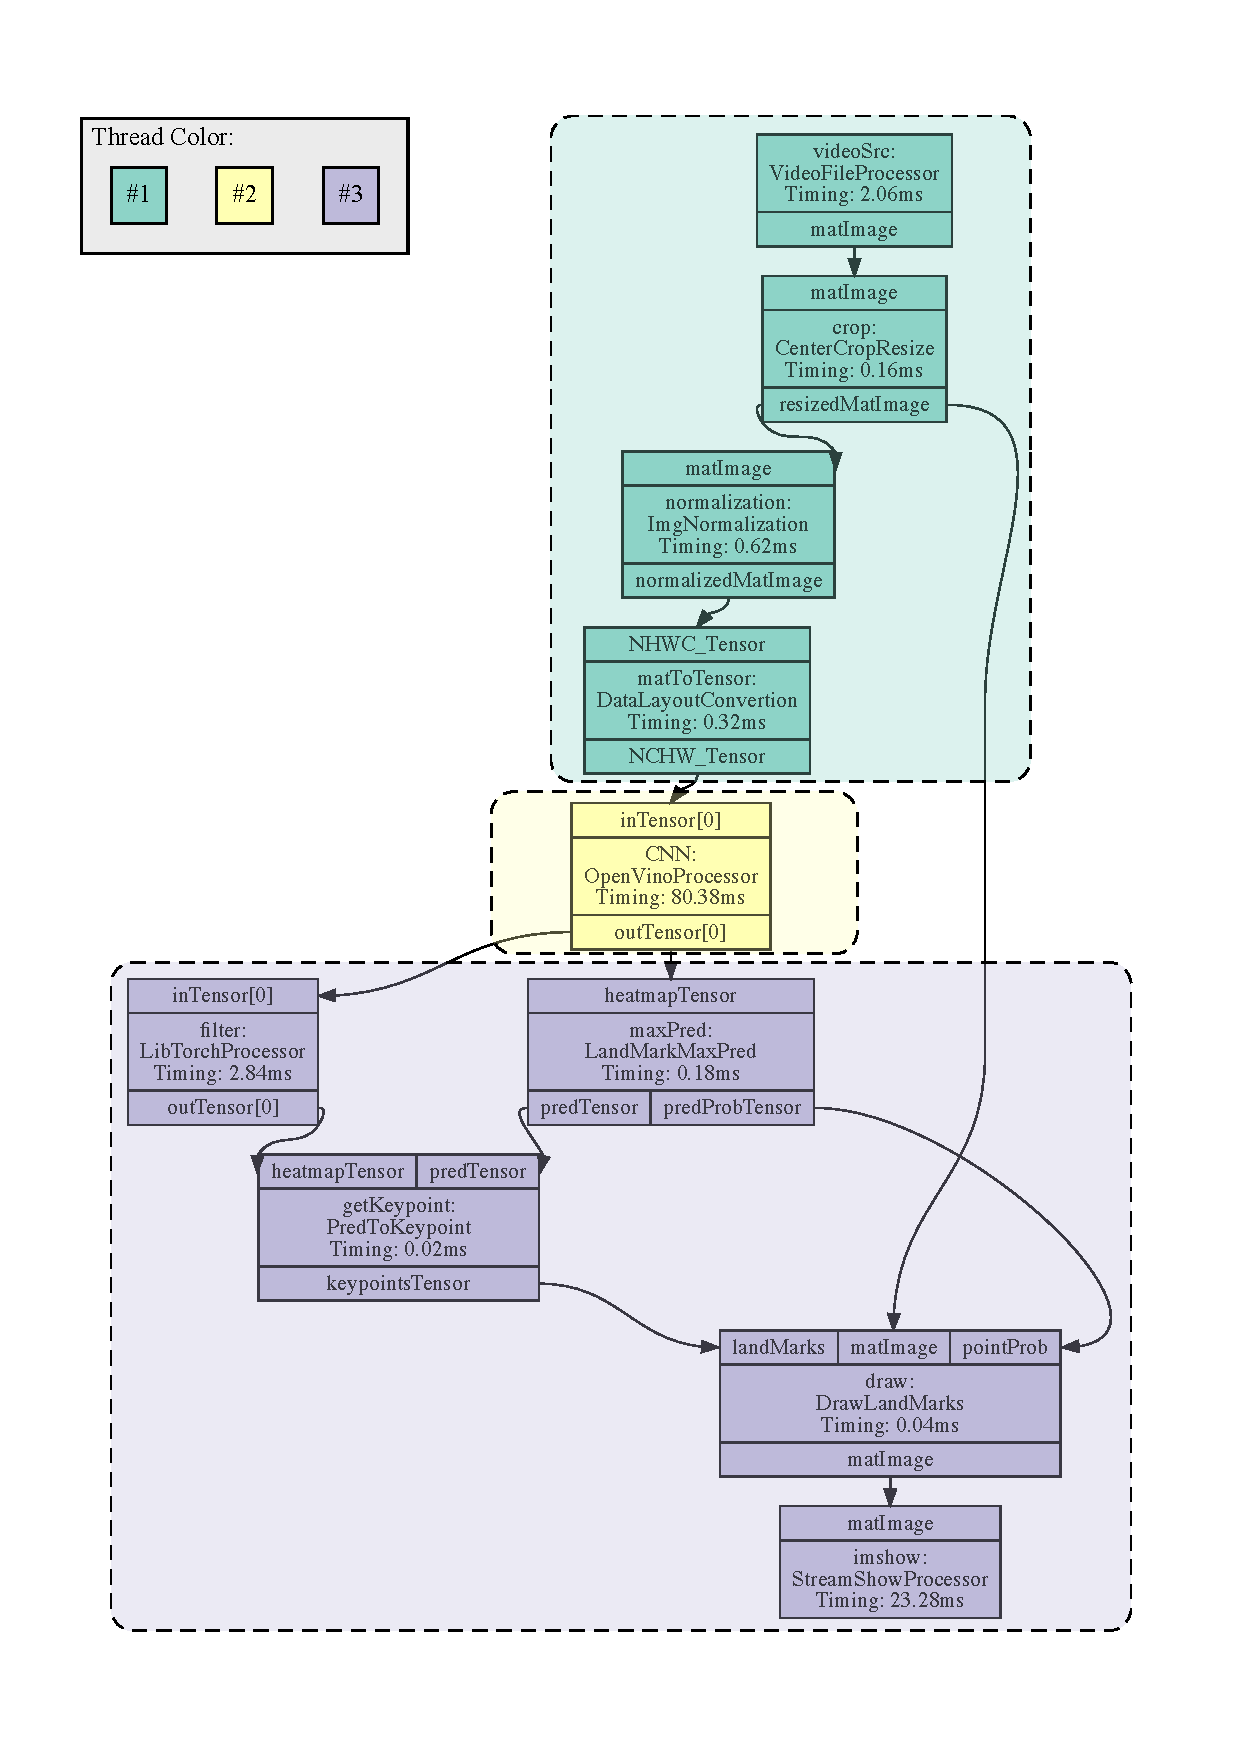
\includegraphics[width=0.7\textwidth]{figure/AVP_pose_estimation.pdf}
    \caption[AVPipe可视化DAG流程图的示例]{人体姿态检测视频处理任务在AVPipe框架下处理流程的可视化。不同颜色代表不同的线程。每个节点的上下栏中显示所连接的Stream的标签。节点的中间显示了该计算节点的标签,调用的计算类以及运行时间信息,其中节点的时间信息是通过AVPipe的性能分析工具从Intel i5-8210Y处理器的MacBook Air的预运行结果中获得的。}
    \label{fig:pose_dag}
\end{figure}

接下来是AVPipe的视频流处理任务的性能分析工具。AVPipe作为一个通用的为终端或边缘设备提供视频流处理任务部署的框架,对处理流程的运行性能有着较高的要求。考虑到视频流处理任务在绝大多数情况下并不会造成计算资源的满负荷运行,并且运行耗时在视频处理任务中更为敏感,我们在AVPipe的性能分析上主要关注在处理流程中各个计算模块的实际计算耗时。为了获得较为准确的各个处理步骤在真实场景下的运行耗时,我们采用预运行(Pre-execution\cite{kim2002design})的方式进行计算模块运行信息的采集,即通过AVPipe的代码生成工具生成一个专门用于运行测试的只会运行较少帧数(如50或100帧)的,包含运行信息报告的C++任务代码。AVPipe的C++代码库中包含有运行计时相关的代码,这部分代码需要在编译时添加必要的宏定义才会有效,在平常情况下这部分代码是不会进行编译的。代码生成工具会为测试代码用到的CMake配置文件添加必要的宏定义,使得最终的运行结果会输出各计算模块在预运行测试帧上的平均处理耗时。
图\ref{fig:pose_dag}中也显示了每个计算模块的具体耗时信息,我们可以直观看到CNN推理模块是整个处理流中最为耗时的模块。在下一小节中我们将会对AVPipe提供的自动优化策略做一介绍。

%图\ref{fig:pose_dag}实际上是由多线程优化工具在在完成线程分配后,调用AVPipe的可视化工具得到的。
% 甘特图 @TODO

\subsection{性能分析驱动的多线程优化}
利用\ref{ch4:viz_prof}中介绍的性能分析工具,我们可以得到每个计算模块的运行耗时信息,利用这一信息,我们可以较容易地分析得到整个处理流程中的瓶颈在哪些处理步骤上。
我们采取多线程优化是为了提高计算资源的利用率,加快视频处理的速度。就AVPipe所涉及的优化层面来讲,我们的优化是存在理论上界的,即每帧的处理耗时是不会低于整个处理流程中最耗时计算模块的用时,再深入的模块优化目前并不属于本课题的研究内容。因此,我们的多线程优化也有了一个较明确的目标:尽可能使AVPipe中的视频流任务的处理速度逼近理论上界。在实现策略上,我们通过多级流水线模型,DAG多分支并行等策略尽可能使其他的计算模块在瓶颈模块在运行的同时完成运行,以此达到掩藏非瓶颈模块计算耗时的目的。
AVPipe的多线程优化工具会依据其启发式算法同时考虑DAG流程图的并行优化与多阶段流水线(Pipeline)并行优化,我们将在本节接下来的讨论中对该算法进行具体介绍。\par

算法\ref{algo:opti}列出了AVPipe所使用的多线程优化算法(auto\_multi\_threading,简称autoMT)的伪代码,我们将在此对算法\ref{algo:opti}做必要的解释于说明。在\ref{ch2:dag_sched}我们已经提过对DAG任务的划分于调度是NP-Complete问题,需要针对具体任务设计相应的启发式算法。在这里我们的autoMT既参考了依据运行时长与拓扑排序的静态节点调度策略,又利用了基于层级聚类方法的DAG划分策略。
其大体思路是:在满足给定的线程数量限制的情况下,我们不断地从待优化的线程列表中选出最耗时线程,再从最耗时线程中选出最耗时计算模块,判断这些模块的耗时。对于用时大于某一阈值$thresh$的模块,我们会尽可能地将其分配到单独的线程中;对用时小于$thresh$的模块,我们会使该模块不断与其周围邻近有依赖的计算模块进行合并构成一个有一定规模的计算模块集合,再将这些计算模块放入同一线程中。上述算法思路基本体现了一个启发式的贪心策略,由于我们所涉及的数据处理流程图的规模还是较小(多数情况下不超过20个节点),不太会使贪心算法陷入较为复杂的局部解中,因此autoMT贪心策略的有效性是有一定保障的。
在了解了优化算法的主体思路后,我们还需要对算法实现的几个关键点结合伪代码\ref{algo:opti}进行讨论:
\begin{enumerate}[wide]
    \item max \#threads。我们可以在autoMT算法中设置可以使用的最多线程数量,对多核处理器来说,其能真正同时运行的线程数量的上限取决于处理器核心的个数,一般情况下只需将最大线程数量设置为处理器的核心数即可。需要注意的是,最大线程数量只是为AVPipe视频处理任务可使用线程数规定了上限,优化后实际所用到的线程数也有可能会少于最大可用线程数,因为现有的线程已经可以实现了非瓶颈计算模块的用时掩盖,更多的线程并不会为任务的性能带来提升,反而会引入额外的线程管理开销。
    \item time threshold ratio。
    \item 线程邻近依赖节点的定义。
\end{enumerate}


\begin{algorithm}[htb]
  \caption{多线程优化算法 auto\_multi\_threading}
  \label{algo:opti}
  \small
%   \SetAlgoLined
  \SetNoFillComment
  \SetKwInOut{Input}{Input}\SetKwInOut{Output}{Output}
  \Input{task DAG $G=(V,E)$, max \#threads $MT$, time threshold ratio $ratio$}
  \Output{a thread list of sets of computing components $threads$}
  
  \tcc{do the initialization}
  $tmpThreads := [G.topoOrderings]$ \tcp*{temporary thread list to be selected}
  $setThreads := []$ \tcp*{a set of the selected, optimized threads}
  $threads := []$\;
%   \tcc{get the time threshold}
  \eIf{$ratio$ is set}  
    {$thresh = G.totalTime \times ratio$}
    {$thresh = \max(V.\text{timing})$}
  
  \While{|tmpThreads|+|setThreads|<MT {\bf and} \#threads is increasing}{
    take the most time consuming thread $T_x$ out of $tmpThreads$\;
    \If{$T_x$.timing < $thresh$}{$setThreads$.append($T_x$);\quad continue\;}
    select the most time consuming component $v_x$ from $T_x$\;
    $predecessors :=$ list of predecessor components of $v_x$ in $T_x$ by topo-order\;
    $successors :=$ list of successor components of $v_x$ in $T_x$ by topo-order\;
    $unrelated := T_x - predecessors - successors$\;
    
    $T_{new} := [v_x]$\;
    \If{\#threads left $\leq$ 3}{
        $T_{tmp} := T_{new}$\;
        \While{$T_{tmp}$.timing < $thresh$}{
            $T_{new} := T_{tmp}$\;
            $V_{dep} := \{v \in T_x | \exists u \in T_{new}, u \text{ has direct connection to } v\}$\; \label{algo:caveat!}
            % sort $V_{dep}$ according to timing by descending order\;
            % \For{$v_i \in V_{dep}$}{}
            $candidate :=$ most time consuming component in $V_{dep}$\;
            \eIf{candidate is not Null}
            {
                $T_{tmp}$.append($candidate$)\; 
                remove $candidate$ from $predecessors$ or $successors$\;
            }
            {
                break\;
            }
        }
        \tcp{put with $unrelated$ in a proper list}
        \For{$v_i \in unrelated$}{
            put $v_i$ into the least time consuming one of \{$predecessors, successors, T_{new}$\}\;
        }
        $setThreads$.append($T_{new}$);\quad$tmpThreads$.append($predecessors, successors$)\;
    }
    \If{\#threads left = 2}{
        % \tcp{put with $unrelated$ in a proper list}
        \For{$v_i \in unrelated$}{
            put $v_i$ into the least time consuming one of \{$predecessors, successors, T_{new}$\}\;
        }
        \tcc{thread combining}
        $T_{new} := T_{new} + $  less time consuming one between $predecessors$, $successors$\;
        $T_{side} := $ more time consuming one between $predecessors$, $successors$\;
        $setThreads$.append($T_{new}$);\quad$tmpThreads$.append($T_{side}$)\;
    }
    \tcc{\#threads left = 1 will not happen}
  }
  $threads := setThreads + tmpThreads$\;
  \Return $threads$\;
\end{algorithm}

% 异构场景下的计算资源分配与调度 看进度加
